\begin{center}
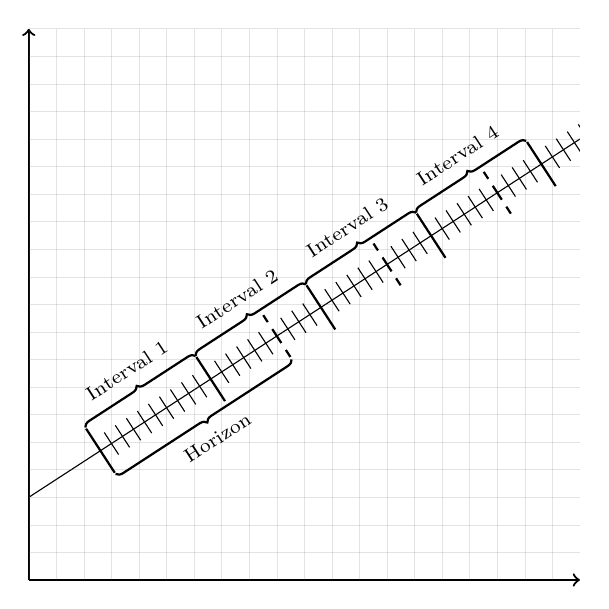
\begin{tikzpicture}
	[scale=7,
	axis/.style={->,black,thick}]

	% Draw main axes
	\draw[axis] (0,0) -- (1,0);
	\draw[axis] (0,0) -- (0,1);
	
	\clip (0,0) rectangle (1, 1);
	
	\draw[] (0,0.15) -- (1,0.8);
	
	% Draw grid
	\foreach \x in {0,0.05,...,1.05}
		\foreach \y in {0,0.05,...,1.05}
		{
			\draw[very thin, gray, opacity=0.01] (\x, 0) -- (\x, 1);
			\draw[very thin, gray, opacity=0.01] (0, \y) -- (1, \y);
		}
	
	\foreach \x/\y in {0.13/0.2345, 0.15/0.2475, 0.17/0.2605, 0.19/0.2735, 0.21/0.2865, 0.23/0.2995,
					   0.25/0.3125, 0.27/0.3255, 0.29/0.3385, 0.31/0.3515, 0.33/0.3645, 0.35/0.3775,
					   0.37/0.3905, 0.39/0.4035, 0.41/0.4165, 0.43/0.4295, 0.47/0.4555, 0.49/0.4685,
					   0.51/0.4815, 0.53/0.4945, 0.55/0.5075, 0.57/0.5205, 0.59/0.5335, 0.61/0.5465,
					   0.63/0.5595, 0.67/0.5855, 0.69/0.5985, 0.71/0.6115, 0.73/0.6245, 0.75/0.6375,
					   0.77/0.6505, 0.79/0.6635, 0.81/0.6765, 0.83/0.6895, 0.87/0.7155, 0.89/0.7285,
					   0.91/0.7415, 0.93/0.7545, 0.95/0.7675, 0.97/0.7805, 0.99/0.7935, 1.01/0.8065}
	{
		\draw[thin] (\x,\y) -- (\x+0.065*0.2, \y-0.1*0.2);
		\draw[thin] (\x,\y) -- (\x-0.065*0.2, \y+0.1*0.2);
	}
	
	\foreach \x/\y in {0.13/0.2345, 0.33/0.3645, 0.53/0.4945, 0.73/0.6245, 0.93/0.7545}
	{
		\draw[thick] (\x,\y) -- (\x+0.065*0.4, \y-0.1*0.4);
		\draw[thick] (\x,\y) -- (\x-0.065*0.4, \y+0.1*0.4);
	}
	
	\foreach \x/\y in {0.45/0.4425, 0.65/0.5725, 0.85/0.7025}
	{
		\draw[dashed, thick] (\x,\y) -- (\x+0.065*0.4, \y-0.1*0.4);
		\draw[dashed, thick] (\x,\y) -- (\x-0.065*0.4, \y+0.1*0.4);
	}
	
	\draw[thick, decoration={brace, raise=10pt}, decorate]
		(0.13, 0.2345) -- (0.33, 0.3645) node[midway, above=13pt, sloped] {\scriptsize Interval 1};
		
	\draw[thick, decoration={brace, raise=10pt}, decorate]
		(0.33, 0.3645) -- (0.53, 0.4945) node[midway, above=13pt, sloped] {\scriptsize Interval 2};
	
	\draw[thick, decoration={brace, raise=10pt}, decorate]
		(0.53, 0.4945) -- (0.73, 0.6245) node[midway, above=13pt, sloped] {\scriptsize Interval 3};

	\draw[thick, decoration={brace, raise=10pt}, decorate]
		(0.73, 0.6245) -- (0.93, 0.7545) node[midway, above=13pt, sloped] {\scriptsize Interval 4};
	
	\draw[thick, decoration={brace, mirror, raise=10pt}, decorate]
		(0.13, 0.2345) -- (0.45, 0.4425) node[midway, below=13pt, sloped] {\scriptsize Horizon};
	
	
	%\begin{scope}[on background layer]
	%	\fill[gray, opacity=.9] (0.13+0.065*0.4, 0.2345-0.1*0.4) -- (0.33+0.065*0.4, 0.3645-0.1*0.4) -- (0.33-0.065*0.4, 0.3645+0.1*0.4) -- (0.13-0.065*0.4, 0.2345+0.1*0.4);
	%\end{scope}
	
	%\begin{scope}[on background layer]
	%	\fill[gray, opacity=.7] (0.33+0.065*0.4, 0.3645-0.1*0.4) -- (0.53+0.065*0.4, 0.4945-0.1*0.4) -- (0.53-0.065*0.4, 0.4945+0.1*0.4) -- (0.33-0.065*0.4, 0.3645+0.1*0.4);
	%\end{scope}
	
	%\begin{scope}[on background layer]
	%	\fill[gray, opacity=.5] (0.53+0.065*0.4, 0.4945-0.1*0.4) -- (0.73+0.065*0.4, 0.6245-0.1*0.4) -- (0.73-0.065*0.4, 0.6245+0.1*0.4) -- (0.53-0.065*0.4, 0.4945+0.1*0.4);
	%\end{scope}
	
	%\begin{scope}[on background layer]
	%	\fill[black, opacity=.2] (0.73+0.065*0.4, 0.6245-0.1*0.4) -- (0.93+0.065*0.4, 0.7545-0.1*0.4) -- (0.93-0.065*0.4, 0.7545+0.1*0.4) -- (0.73-0.065*0.4, 0.6245+0.1*0.4);
	%\end{scope}
	
	
\end{tikzpicture}
\end{center}